\documentclass{emulateapj}
%\documentclass[11pt,preprint]{aastex}
%% preprint2 produces a double-column, single-spaced document:
%\documentclass{emulateapj}
%\documentclass[preprint2]{aastex}


\bibliographystyle{apj}
\usepackage{epsfig,graphicx}
\usepackage{amsmath}
\usepackage{natbib}
\usepackage{lscape}
\usepackage{comment}
\usepackage{threeparttable}

\begin{document}

\title{The 300 km~s$^{-1}$ stellar stream near Segue\,1: Insights From High-Resolution Spectroscopy of its brightest star}
\author{Ragnhild Lunnan$^1$,  Anna Frebel$^1$, John E. Norris$^2$, Rosemary F. G. Wyse$^3$ and Gerard Gilmore$^4$}
\affil{$^1$ Harvard-Smithsonian Center for Astrophysics, 60 Garden Street, Cambridge, MA 02138, USA}
\affil{$^2$ Research School of Astronomy \& Astrophysics, The Australian National University, Mount Stromlo Observatory, Cotter Road, Weston, ACT 2611, Australia}
\affil{$^3$ The Johns Hopkins University, Department of Physics \& Astronomy, 300 N. Charles Street, Baltimore, MD 21218, USA}
\affil{$^4$ Institute of Astronomy, University of Cambridge, Madingley Road, Cambridge CB3 0HA, UK}
\email{rlunnan@cfa.harvard.edu}


\begin{abstract}
In kinematic surveys of the faint satellite galaxy Segue\,1, an overdensity of stars with velocities around 300~km~s$^{-1}$ has been seen, first seen in \citet{Geha2009} and interpreted as a possible stellar stream. We present a high-resolution spectrum and abundance analysis of Segue1-11, the brightest likely stream member star from the kinematic sample of \citet{Norris2010a}. We determine a metallicity of [Fe/H] $ = -1.44 \pm XX$ for Segue1-11, and find abundance patterns similar to typical halo stars at this metallicity. Comparing our stellar parameter solution to theoretical isochrones, we estimate a distance of $18 \pm 7$ kpc. Both the metallicity and distance estimates are in good agreement with what can be inferred from comparing the SDSS photometric data of the stream stars to globular cluster sequences. While several other structures overlap with the stream in this part of the sky, the combination of kinematic, chemical and distance information makes it unlikely that these stars are associated with either the Segue\,1 galaxy, the Sagittarius stream or the Orphan stream.

\end{abstract}


\keywords{Galaxy: halo -- Galaxy: kinematics and dynamics -- stars: abundances}


%%%%%%%%%%%%%%%%%%%%%%%%%%%%%%%%%%%%%%%%%%%%%%%%%%%%%%%%%%%%%%%%%%%%%%%%%%%%%%%%%%%%%%%%%%%%%%%%%%%%%%

\section{Introduction}
\label{sec:intro}
 

In the $\Lambda$CDM model, structure builds up hierarchically, with smaller objects merging to build larger ones. One consequence of this is stellar streams in the galactic halo, produced as accreted objects are tidally disrupted (see e.g. \citealt{Lynden-Bell1995} and references therein). A well-known example is the stream extending from the Sagittarius dwarf spheroidal, which has been traced more than one full wrap around the Milky Way \citep[e.g.][]{Ibata1994, Majewski2003}. In a part of the sky dubbed the ``Field of Streams'' \citep{Belokurov2006b}, at least two wraps of the Sagittarius stream as well as several other structures are visible.

A new velocity structure in this field has recently been discovered overlapping with the ultra-faint object Segue\,1 \citep{Belokurov2007}: Radial velocity data to determine Segue\,1's velocity dispersion by \citet{Geha2009} revealed a group of stars moving near 300~km~s$^{-1}$. The same overdensity of stars at this velocity was seen by Norris et al. (2010; hereafter N10)\nocite{Norris2010a}, who targeted Segue\,1 stars in the RGB locus, and in the larger spectroscopic sample of Segue\,1 stars of Simon et al. (2011; hereafter S11)\nocite{Simon2011}. The stars have so far been interpreted as part of a stellar stream, and we shall refer to it as the ``300~km~s$^{-1}$ stream'' throughout this paper. Since the full extent of this structure has not been mapped out, however, we note that it is also possible these stars belong to a bound object.

From SDSS photometry, one can get an estimate of the distance and metallicity of the stream by comparing the color-magnitude diagram to globular cluster sequences and isochrones. To further characterize the stream chemically, however, high-resolution spectroscopy is necessary. Here, we present the first high-resolution spectrum and detailed abundance analysis of a star in the 300~km~s$^{-1}$ stream.

This paper is organized as follows. We briefly discuss the sample from which the main target for high-resolution spectroscopy was selected in Section~\ref{sec:medres}. The observations and basic data analysis of our target star is presented in Section~\ref{sec:obs}, and the abundance analysis in Section~\ref{sec:abund}. We interpret the results and discuss the nature and potential origin of the stream in Section~\ref{sec:char}. Our conclusions are summarized in Section~\ref{sec:conc}.
%%%%%%%%%%%%%%%%%%%%%%%%%%%%%%%%%%%%%%%%%%%%%%%%%%%%%%%%%%%%%%%%%%%%%%%%%%%%%%%%%%%%%%%%%%%%%%%%%%%%%%
\section{Stream sample and target selection}
\label{sec:medres}


There are two existing medium-resolution spectroscopic studies of the region around Segue\,1, N10 and S11. N10's data was obtained with the Anglo-Australian Telescope's AAOmega spectrograph, which can take simultaneous spectra of 400 targets over a field 2$^{\circ}$ in diameter. They were targeting stars in the RGB locus. S11, on the other hand, were using the {\small DEIMOS} spectrograph on the KeckII telescope, focusing on an area within $\sim 15$\arcmin of the center of Segue\,1, and going deeper than N10. Table~\ref{tab:members} lists all stars (52 total) in the two samples with heliocentric radial velocities higher than 240~km~s$^{-1}$, i.e. stars with higher velocities than consistent with Segue\,1 membership and so potential stream candidates. This includes four targets from the AAOmega sample not published in N10 due to slightly lower confidence in the radial velocity measurement. All photometry is from the Sloan Digital Sky Survey, DR7 \citep{Abazajian2009}. The estimated velocity uncertainty for the N10 stars is 10~km~s$^{-1}$; the individual velocity uncertainties for S11 stars are shown in the table.

Figure~\ref{fig:col_mag} summarizes the properties of the two samples. The top left panel shows a histogram of the heliocentric radial velocities measured. The central peak ($\sim$ 270-330~km~s$^{-1}$) has a mean velocity of $300.4 \pm 1.1 \mbox{km s}^{-1}$ and a dispersion of $10.3 \pm 1.2 \mbox{km s}^{-1}$. Considering the independent N10 and S11 samples separately we still arrive at a dispersion of 10~km~s$^{-1}$ for the central peak, and similar means ($303.3 \pm 3$~km~s$^{-1}$ for N10 versus $299.1 \pm 1$~km~s$^{-1}$ for S11). It is not clear whether the intermediate ``bridge'' candidates with 240~km~s$^{-1}$ $< v_{helio} < $270~km~s~$^{-1}$ or the three extreme-velocity stars with $v_{helio} > $ 340~km~s$^{-1}$ should be considered part of the same structure, but follow-up observations tracing the stream over a larger field of view could resolve this. Either way, the mean velocity of this structure is extreme, and the dispersion is resolved and high -- it is not a cold stream.

The top right panel of Fig.~\ref{fig:col_mag} shows the color-magnitude diagram of all the stream candidate stars from Table~\ref{tab:members}. Here, stream candidates are shown as black circles. (Three stars redder than $(g-i) = 1.2 $ are not shown.) For comparison, the green triangles show radial velocity members of the Segue\,1 dwarf galaxy, which was the target of the N10 and S11 studies. Open symbols show stars from the N10/AAO sample, while filled symbols are from the S11 sample. Note that the N10 sample covers a much larger field of view but does not go as deep -- as a result, most of the bright stream stars, including our target (star symbol), show up in this sample. In order to illustrate the photometric criteria used in the samples, the blue and red dots show the stars observed by N10 and S11, respectively, that met their photometric selection cut for follow-up spectroscopy, but are radial velocity non-members of Segue\,1 and the stream.

The solid line shows the M5 cluster sequence \citep{An2008}, which gives a good fit to the stream main sequence and subgiant branch when shifted to a distance of 18~kpc. The metallicity of M5 is [Fe/H] $= -1.3$, and the SDSS photometry suggests that the stream is slightly more metal-rich than Segue\,1 \citep{Simon2011}. The red giant branch of the stream is bluer than this sequence, however, and is better fit by e.g. the RGB of the more metal-poor cluster M92.

There are six stream candidate stars brighter than $r = 19$, and thus possible candidates for high-resolution spectroscopy. Our chosen target (SDSSJ100914.95+155948.4; the first star in Table~\ref{tab:members}) is marked with an open star symbol. It is identified as ``Segue1-11'' in N10, and we shall refer to it by this designation throughout the paper. Its location in the color-magnitude diagram indicates that it is most likely a red giant, though it could also be consistent with a horizontal branch at this distance. Both its colors, and the radial velocity of 301~km~s$^{-1}$ measured by N10 are consistent with stream membership. The medium-resolution spectrum indicated a metallicity of [Fe/H]$\simeq -0.7$. Accordingly, we deemed it the best candidate for high-resolution spectroscopy follow-up. 

The nature of the other five bright stars is less clear. As noted in \citet{Geha2009}, random halo stars at these extreme velocities are very rare. If they indeed were turnoff stars, the stream would have a coherent velocity over four magnitudes in distance modulus, which also seems unlikely given orbits. The three stars around $r\sim 17.5$ could be RHB stars, but if so raises the question of why we do not see the expected, more numerous red giants. The nature of the very bright star at $r = 15.8$ is also not understood. To resolve these questions, getting spectra of these brighter stars could provide more insight. 

Finally, the spatial coverage of the two samples is shown in the two bottom panels. The brighter stream stars in the N10 sample (left) extend at least over 1$^{\circ}$ on the sky; the deeper sample of S11 (right) only covers a 15\arcmin radius around the center of Segue\,1. The box size here represents the full field of view observed in the N10 sample, and so for the lower left panels, again, all stars observed by N10 are shown to better illustrate the distribution. Follow-up observations to determine the full extent of this stream on the sky, as well as deeper observations in a larger region than that covered by S11, would be very important for better understanding and characterizing this structure.



\begin{deluxetable*}{lcccccccc}
\tabletypesize{\scriptsize}
\tablecaption{Stream Member Candidate Stars\label{tab:members}}
\tablehead{
	\colhead{Identifier} &
	\colhead{R. A.} &
	\colhead{Dec.} &
	\colhead{$g$} &
	\colhead{$r$} &
	\colhead{$i$} &
	\colhead{$g \-- r$} &
	\colhead{$V_{hel}$} &
	\colhead{Ref} \\
  & (J2000) & (J2000) & & & & & (km s$^{-1}$) &  
}
\startdata
300S-1\tablenotemark{a} & 10\phn09\phn15.0 & $+$15\phn59\phn48.4 &  17.99 & 17.49 & 17.26 & 0.73 & 307 & N10 \\
300S-2 & 10\phn07\phn40.1 & $+$16\phn03\phn09.7 &  19.96 & 19.55 & 19.44 & 0.52 & 298 & N10, S11    \\
300S-3 & 10\phn06\phn59.0 & $+$15\phn44\phn18.8 &  19.72 & 19.33 & 19.14 & 0.58 & 307 & N10     \\
300S-4 & 10\phn06\phn51.8 & $+$15\phn49\phn41.5 &  20.36 & 20.04 & 19.91 & 0.45 & 300 & AAO     \\
300S-5 & 10\phn06\phn20.0 & $+$15\phn46\phn12.7 &  20.09 & 19.78 & 19.67 & 0.42 & 315 & AAO     \\
300S-6 & 10\phn06\phn12.0 & $+$15\phn45\phn48.4 &  20.08 & 19.62 & 19.61 & 0.47 & 327 & N10     \\
300S-7 & 10\phn05\phn30.6 & $+$15\phn54\phn18.1 &  19.83 & 19.49 & 19.31 & 0.52 & 305 & N10     \\
300S-8 & 10\phn06\phn27.7 & $+$15\phn54\phn08.6 &  20.15 & 19.88 & 19.71 & 0.44 & 300 & AAO     \\
300S-9 & 10\phn06\phn47.7 & $+$16\phn13\phn30.1 &  20.01 & 19.70 & 19.51 & 0.50 & 300 & AAO     \\
300S-10 & 10\phn06\phn58.5 & $+$16\phn20\phn45.6 &  19.84 & 19.37 & 19.18 & 0.66 & 295 & N10     \\
300S-11 & 10\phn08\phn39.7 & $+$16\phn28\phn26.7 &  19.16 & 18.73 & 18.60 & 0.56 & 288 & N10     \\
300S-12 & 10\phn06\phn00.2 & $+$16\phn05\phn18.6 &  20.22 & 19.68 & 19.51 & 0.71 & 242 & N10      \\
300S-13 & 10\phn06\phn18.7 & $+$16\phn03\phn39.0 &  21.67 & 21.14 & 20.90 & 0.77 & 268.6  $\pm$\phn3.1 & S11     \\
300S-14 & 10\phn06\phn20.0 & $+$16\phn00\phn42.1 &  21.70 & 21.41 & 21.18 & 0.52 & 305.5  $\pm$\phn4.3 & S11     \\
300S-15 & 10\phn06\phn30.9 & $+$16\phn15\phn12.1 &  21.47 & 21.13 & 20.95 & 0.52 & 321.0  $\pm$\phn8.8 & S11     \\
300S-16 & 10\phn06\phn42.8 & $+$15\phn57\phn09.3 &  21.56 & 21.23 & 21.02 & 0.54 & 291.9  $\pm$\phn6.4 & S11     \\
300S-17 & 10\phn06\phn46.8 & $+$16\phn06\phn08.3 &  20.53 & 20.22 & 20.07 & 0.46 & 294.5  $\pm$\phn2.9 & S11     \\
300S-18 & 10\phn06\phn48.5 & $+$16\phn09\phn58.1 &  20.27 & 19.98 & 19.79 & 0.48 & 306.0  $\pm$\phn2.6 & S11     \\
300S-19 & 10\phn06\phn50.8 & $+$16\phn03\phn51.2 &  22.13 & 21.95 & 21.83 & 0.30 & 312.6  $\pm$11.9 & G09, S11     \\
300S-20 & 10\phn06\phn54.2 & $+$15\phn55\phn20.7 &  22.12 & 21.53 & 21.29 & 0.83 & 268.5  $\pm$\phn6.2 & S11     \\
300S-21 & 10\phn06\phn56.1 & $+$16\phn06\phn60.0 &  21.34 & 21.09 & 20.99 & 0.35 & 302.0  $\pm$\phn2.6 & S11     \\
300S-22 & 10\phn06\phn58.5 & $+$15\phn57\phn48.9 &  21.56 & 21.09 & 20.84 & 0.72 & 290.5  $\pm$\phn3.6 & S11     \\
300S-23 & 10\phn07\phn04.6 & $+$16\phn01\phn30.8 &  21.22 & 20.81 & 20.76 & 0.46 & 295.8  $\pm$\phn3.9 & S11     \\
300S-24 & 10\phn07\phn04.6 & $+$16\phn08\phn12.6 &  21.08 & 20.85 & 20.74 & 0.34 & 296.9  $\pm$\phn3.4 & S11     \\
300S-25 & 10\phn07\phn08.4 & $+$15\phn56\phn46.3 &  22.03 & 21.56 & 21.45 & 0.58 & 286.3  $\pm$\phn5.4 & S11     \\
300S-26 & 10\phn07\phn09.1 & $+$16\phn04\phn36.6 &  22.29 & 21.88 & 21.57 & 0.72 & 312.7  $\pm$\phn6.4 & S11     \\
300S-27 & 10\phn07\phn09.7 & $+$15\phn53\phn12.3 &  16.11 & 15.83 & 15.72 & 0.39 & 303.4  $\pm$\phn2.2 & S11     \\
300S-28 & 10\phn07\phn13.0 & $+$15\phn57\phn34.8 &  18.28 & 18.00 & 17.87 & 0.41 & 307.9  $\pm$\phn2.4 & S11     \\
300S-29 & 10\phn07\phn13.7 & $+$16\phn04\phn44.8 &  22.13 & 21.76 & 21.47 & 0.66 & 293.4  $\pm$\phn4.8 & G09, S11     \\
300S-30 & 10\phn07\phn15.5 & $+$16\phn05\phn52.1 &  20.36 & 20.07 & 19.97 & 0.39 & 282.0  $\pm$\phn2.8 & S11     \\
300S-31 & 10\phn07\phn15.5 & $+$16\phn15\phn19.1 &  20.74 & 20.43 & 20.42 & 0.32 & 266.8  $\pm$\phn3.1 & S11     \\
300S-32 & 10\phn07\phn17.2 & $+$16\phn05\phn11.9 &  22.10 & 21.78 & 21.38 & 0.72 & 266.3  $\pm$\phn4.4 & S11     \\
300S-33 & 10\phn07\phn17.4 & $+$16\phn03\phn55.6 &  20.11 & 19.77 & 19.64 & 0.47 & 295.9  $\pm$\phn2.4 & G09, S11    \\
300S-34 & 10\phn07\phn20.0 & $+$16\phn01\phn37.5 &  17.62 & 17.27 & 17.12 & 0.50 & 312.7  $\pm$\phn2.2 & S11     \\
300S-35 & 10\phn07\phn21.2 & $+$16\phn11\phn18.2 &  20.99 & 19.73 & 19.20 & 1.79 & 281.6  $\pm$\phn2.4 & S11     \\
300S-36 & 10\phn07\phn21.8 & $+$15\phn54\phn24.5 &  20.61 & 20.22 & 20.22 & 0.39 & 307.2  $\pm$\phn5.5 & S11     \\
300S-37 & 10\phn07\phn29.6 & $+$16\phn11\phn07.1 &  20.35 & 19.34 & 19.02 & 1.33 & 309.6  $\pm$\phn2.2 & S11     \\
300S-38 & 10\phn07\phn32.5 & $+$16\phn05\phn00.5 &  22.58 & 22.04 & 21.91 & 0.67 & 281.1  $\pm$\phn6.9 & G09, S11     \\
300S-39 & 10\phn07\phn35.0 & $+$15\phn54\phn31.5 &  20.78 & 20.54 & 20.39 & 0.39 & 303.2  $\pm$\phn2.8 & S11     \\
300S-40 & 10\phn07\phn37.3 & $+$16\phn07\phn46.2 &  21.25 & 20.99 & 20.81 & 0.44 & 296.0  $\pm$\phn3.9 & S11     \\
300S-41 & 10\phn07\phn40.2 & $+$15\phn58\phn55.6 &  21.32 & 20.96 & 20.80 & 0.52 & 295.8  $\pm$\phn3.8 & S11     \\
300S-42 & 10\phn07\phn42.5 & $+$16\phn00\phn06.8 &  22.47 & 22.02 & 21.46 & 1.01 & 296.6  $\pm$10.3 & S11     \\
300S-43 & 10\phn07\phn43.8 & $+$15\phn49\phn32.9 &  22.47 & 20.98 & 20.36 & 2.11 & 299.2  $\pm$\phn2.5 & S11     \\
300S-44 & 10\phn07\phn47.2 & $+$16\phn05\phn45.5 &  20.13 & 19.77 & 19.67 & 0.46 & 294.3  $\pm$\phn2.4 & S11     \\
300S-45 & 10\phn07\phn35.9 & $+$16\phn11\phn25.7 &  23.79 & 22.08 & 22.00 & 1.79 & 242.2  $\pm$\phn7.8 & S11     \\
300S-46 & 10\phn06\phn25.7 & $+$15\phn54\phn22.1 &  21.58 & 21.13 & 20.95 & 0.63 & 244.3  $\pm$\phn5.6 & S11     \\
300S-47 & 10\phn07\phn11.8 & $+$16\phn06\phn30.4 &  22.80 & 22.16 & 21.95 & 0.85 & 247.1  $\pm$15.9 & S11     \\
300S-48 & 10\phn07\phn07.8 & $+$16\phn07\phn21.5 &  20.64 & 20.34 & 20.23 & 0.41 & 247.7  $\pm$\phn2.8 & S11     \\
300S-49 & 10\phn07\phn35.2 & $+$15\phn57\phn15.3 &  22.53 & 21.13 & 20.41 & 2.12 & 255.1  $\pm$\phn3.0 & S11     \\
300S-50 & 10\phn06\phn28.4 & $+$15\phn56\phn28.8 &  17.85 & 17.56 & 17.43 & 0.42 & 347.1  $\pm$\phn2.9 & S11     \\
300S-51 & 10\phn07\phn36.9 & $+$15\phn59\phn58.9 &  21.99 & 21.87 & 21.60 & 0.39 & 373.0  $\pm$\phn6.0 & S11     \\
300S-52 & 10\phn06\phn51.7 & $+$16\phn17\phn59.2 &  21.40 & 20.92 & 20.95 & 0.45 & 394.9  $\pm$\phn8.9 & S11 
\enddata
\tablenotetext{a}{Target star, referenced as Segue1-11 in N10}
\end{deluxetable*}

\begin{figure*}
 \begin{center}
  \begin{tabular}{cc}
    \includegraphics[width=8.5cm]{velhist.ps} & \includegraphics[width=8.5cm]{cm_2.ps} \\
    \includegraphics[width=8.5cm]{coord1.ps}  & \includegraphics[width=8.5cm]{coord2.ps}  \\
  \end{tabular}
  \caption{ {\scriptsize Summarizing the properties of the stream star candidates found in N10 and S11. Top left: Heliocentric radial velocity histogram of all stars in the combined N10 and S11 samples with a measured velocity greater than 240~km~s$^{-1}$. The black dashed line shows stars in the N10 sample, the blue dotted lines show stars in the S11 sample, and the solid red line shows the total. Top right: Color-magnitude diagram of the 300~km~s$^{-1}$ stream candidate stars found in S11 (filled circles) and N10 (open circles). The open star symbol denotes our target for high-resolution spectroscopy follow-up. The green triangles show radial velocity members of the ultra-faint dwarf galaxy Segue\,1, which was the target for the spectroscopic studies in which the stream stars were found. Blue (N10) and red (S11) dots show the remainding stars that still meet the photometric cuts in either sample, but are not radial velocity members of Segue\,1 or the stream. Photometry is from the Sloan Digital Sky Survey, DR7 \citep{Abazajian2009}. The black line shows the globular cluster sequence of M5 \citep{An2008}, shifted according to the appropriate reddening for the stream stars, and to a best-fit distance of 18 kpc. Note that this is slightly closer than the $23 \pm 2$ kpc distance of Segue\,1 \citep{Belokurov2007}.    Bottom: coordinate plots of stream candidate stars, showing the N10 sample (left) and S11 sample (right). The box size represents the 2$^{\circ}$ field of view covered by N10 centered on Segue\,1; S11 on the other hand only  observed stars within 15\arcmin of Segue\,1's center. Symbols as in the color-magnitude diagram.} }
  \label{fig:col_mag}
 \end{center}
\end{figure*}





%%%%%%%%%%%%%%%%%%%%%%%%%%%%%%%%%%%%%%%%%%%%%%%%%%%%%%%%%%%%%%%%%%%%%%%%%%%%%%%%%%%%%%%%%%%%%%%%%%%%%%

\section{Observations and Data Analysis}
\label{sec:obs}




\subsection{Observations}

A spectrum of Segue1-11 was obtained with the MIKE spectrograph \citep{mike}
on the Magellan Clay telescope in March 2010. The total exposure time for
this V = 17.6 mag star was 4.5 hours, distributed over six exposures to
 allow for removal of cosmic rays. MIKE spectra have
nearly full optical wavelength coverage from $\sim3500$-9000\,{\AA}. Using
a 1.0\arcsec\, slit and $2\times2$ on-chip binning, a resolution of
$\sim30,000$ is achieved in the red, and $\sim28,000$ in the blue
wavelength regime. 

The data were reduced using an echelle data reduction pipeline made for
MIKE\footnote{Available at http://obs.carnegiescience.edu/Code/python}.
The reduced individual orders were normalized and merged to produce
final one-dimensional blue and red spectra ready for the analysis. The
$S/N$ of the data are 17 at $\sim4500$\,{\AA} and 20 at $\sim5200$\,{\AA}.




In addition to our main target, we also took MIKE spectra of three bright comparison stars chosen from the Fulbright (2000; hereafter F00)\nocite{Fulbright2000} sample in March 2011. These comparison stars were chosen based on having stellar parameters and metallicities that bracketed our first estimate for Segue1-11. Table~\ref{tab:targets} shows the targets, and Table~\ref{tab:segobs} summarizes the observations.  Spectra were taken with a 1.0\arcsec\, slit and short exposures, in order to get a similar data quality and S/N to that of the Segue1-11 spectrum. Fig.~\ref{fig:mglines} shows the spectrum of Segue1-11 and the short-exposure spectra of the comparison stars in the region around the Mg b-lines at 5170\AA. By comparing stellar parameters and abundances derived from these short-exposure spectra to the published values, we obtain another check on our calculated uncertainties.

\begin{deluxetable*}{lcccccccc}
\tabletypesize{\scriptsize}
\tablecaption{Observed Targets \label{tab:targets}}
\tablehead{
	\colhead{Name} &
	\colhead{R. A.} &
	\colhead{Dec.} &
	\colhead{$V$} &
	\colhead{$B \-- V$} & 
	\colhead{UT Date} &
	\colhead{UT Start} &
	\colhead{$t_{exp}$} \\
  & (J2000) & (J2000) & & & & & ($s$)   
}
\startdata  
300S-1     &  10\phn09\phn15.0 &  $+$15\phn59\phn48.4 & 17.70\tablenotemark{a} &  0.68\tablenotemark{a} & 03/08/2010 & 02:35 & 3000 \\
 & & & & & 03/08/2010 & 05:30 & 3600 \\
 & & & & & 03/19/2010 & 05:06 & 3000 \\
 & & & & & 03/22/2010 & 00:37 & 3100 \\
 & & & & & 03/22/2010 & 05:22 & 2800 \\
 & & & & & 03/23/2010 & 05:08 & 700 \\
HIP37335   &  07\phn39\phn50.1 &  $-$01\phn31\phn20.4 & 9.25 &  0.82 & 03/13/2011 & 23:41 & 7      \\
HIP47139   &  09\phn36\phn20.0 &  $-$20\phn53\phn14.8 & 8.34 &  1.01 & 03/12/2011 & 10:08 & 1      \\
HIP68807   &  14\phn05\phn13.0 &  $-$14\phn51\phn25.5 & 7.25 &  0.93 & 03/13/2011 & 23:53 & 5      
\enddata
\tablenotetext{a}{Transformed from SDSS photometry following \citet{Jordi2006}}
\end{deluxetable*}


\begin{figure}
 \begin{center}
  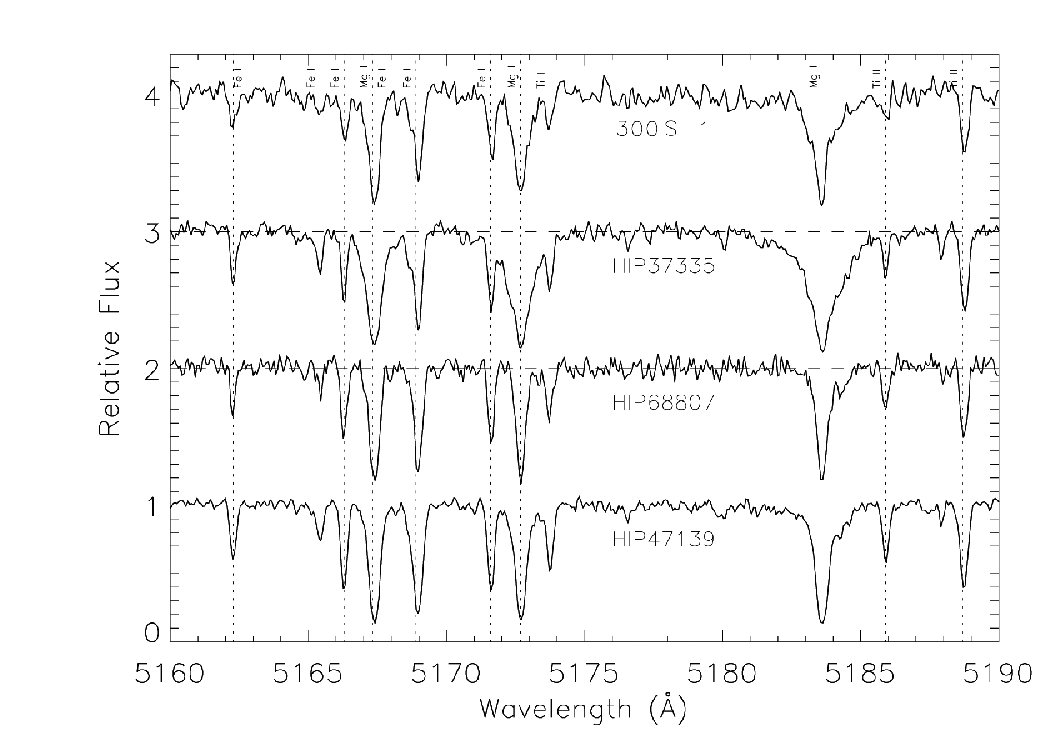
\includegraphics[width=9cm]{Mgspecs_fixed.eps}
  \caption{High-resolution spectrum of our target star, Segue1-11, and the three comparison stars from the F00 sample, in the region around the Mg b-lines. Shown here are the short exposures of the comparison stars, taken to obtain a similar resolution and S/N as the Segue1-11 spectrum.}
  \label{fig:mglines}
 \end{center}
\end{figure}



\subsection{Line Strength Measurements}
\label{sec:linemes}
We obtained a first estimate for the radial velocity from the two strong Mg b lines in the green region of the spectrum, and two additional Mg lines in the blue. Equivalent widths were then measured by fitting Gaussian profiles, and our estimate corrected based on the mean radial velocity from all the lines measured. Using these 366 lines, we find a heliocentric radial velocity of $307.6$~km~s$^{-1}$, with a standard error of the mean of 0.1~km~s$^{-1}$. This is slightly higher than the estimate of $301$~km~s$^{-1}$ from N10 based on the medium resolution spectrum, but consistent within their estimated velocity uncertainty of 10~km~s$^{-1}$. We note that our measurement is well within the estimated range for the 300~km~s$^{-1}$ stream.

The linelist used for the abundance analysis is based on lines presented in \citet{Roederer2010}, \citet{Aoki2007b}, and \citet{Cayrel2004}. In the instances where the same
line was included in more than one (original) linelist, the most up to
date oscillator strength was used, following Roederer et al. (2010).
This linelist was initally compiled for work on stars more metal-poor than
the target, but besides the strongest lines, we found it to
work well for this metallicity range also.


For atomic lines, equivalent widths were measured by fitting Gaussian profiles. Lines with reduced equivalent widths $\log$(EW/$\lambda$) $> -4.5$ were not used for abundance determination, since they fall near the flat part of the curve-of-growth. Given the noise in the spectra, most lines with EW $\lesssim 20$ m\AA\,  were cautiously excluded for abundance determinations.

For molecular features and elements with hyperfine splitting, we used a spectrum synthesis approach. The abundance was then determined by matching synthesized spectra of different abundances to the observed data. See Section~\ref{sec:abund} for details.


\subsection{Stellar Parameters}
\label{sec:stpar}
The stellar parameters were determined by using the iron lines in each spectrum, by an iterative process. First, the microturbulence is fixed by demanding that the line abundances show no trend with reduced equivalent width ($\log \mbox{EW}/\lambda$). Similarly, effective temperature is set by requiring no trend of abundance with excitation potential of the lines. Finally, the gravity is fixed by requiring that the abundance derived from Fe II lines agree with that obtained from Fe I to within 0.05 dex. By varying the temperature and microturbulence, and comparing the slope to the scatter in the data, we adopt an uncertainty of $\pm$ 150 K in temperature, and $\pm$ 0.3~km~s$^{-1}$ in microturbulence. Similarly, we obtain an uncertainty in the gravity of about $\pm$ 0.4 dex by seeing how much gravity can be changed with Fe I and Fe II still being consistent within the scatter.


Table~\ref{tab:comp_para} shows the resulting stellar parameters for Segue1-11 and the three comparison stars obtained with this method, with the values obtained by F00 in parenthesis for comparison. For HIP68807 and HIP47139, our solutions agree well with the parameters published in F00. For HIP37335, we arrive at a slightly higher temperature and gravity, and thus metallicity, than F00.


Figure~\ref{fig:isochr} shows the adopted stellar parameters overplotted with theoretical 10 Gyr isochrones \citep{Kim2002}. Our solution agrees reasonably well with the tracks within their uncertainties. As its position on the color-magnitude diagram suggested, spectroscopically derived stellar parameters confirm that our star is located on the red giant branch.

For comparison, we also use the SDSS colors to determine the temperature photometrically by interpolating the SDSS {\it ugriz} colors to the isochrones from \citet{Kim2002}, using the color tables of Castelli (http://wwwuser.oat.ts.astro.it/castelli/).  This results in a slightly warmer solution (depending on which colors we use), with T$_{\mbox{\small{eff}}} \sim 5400$ K and $\log g \sim 3.5$. If we instead use this set of stellar parameters, we would arrive at [Fe/H] of $-1.3$. This is, however, well within our estimate of uncertainty for the metallicity (see Section~\ref{sec:unc}). For the rest of the analysis, we use the parameters derived from spectroscopy to facilitate the relative analysis with the \citet{Fulbright2000} stars.




\begin{figure}
 \begin{center}
  \includegraphics[width=9cm]{isochrones_10Gyr.ps}
  \caption{Adopted stellar parameters for Segue1-11 (filled star), as well as for the three comparison stars (filled triangles). The open triangles show the values for the comparison stars from Fulbright (2000). Error bars are $\pm$ 150 K and 0.4 dex in $\log g$. Also shown are theoretical 10-Gyr isochrones at [Fe/H] = $-2.5$, $-1.5$ and $-0.5$ respectively \citep{Kim2002}.}
  \label{fig:isochr}
 \end{center}
\end{figure}

\subsection{Model Atmospheres}
Our abundance analysis utilizes one-dimensional plane-parallel Kurucz
model atmospheres with no overshooting \citep{kurucz}. They are computed
under the assumption of local thermodynamic equilibrium (LTE). We use the
2010 version of the MOOG synthesis code (first described in Sneden 1973)\nocite{moog}
for this analysis.  In this version, scattering is currently treated as
true absorption, which may have consequences for abundances derived from
lines in the blue region of the spectrum (see \citet{Frebel2010a} for test on
the matter). Since we have no lines bluer than 4000\,{\AA}, this is, however,
not a serious concern for this analysis.



%%%%%%%%%%%%%%%%%%%%%%%%%%%%%%%%%%%%%%%%%%%%%%%%%%%%%%%%%%%%%%%%%%%%%%%%%%%%%%%%%%%%%%%%%%%%%%%%%%%%%%

\section{Abundance Analysis of Segue1-11}
\label{sec:abund}

The derived stellar abundances of Segue1-11 are summarized in Table~\ref{tab:seg11_abund}. The uncertainties quoted are the standard error of the mean, but we adopt a minimum uncertainty of 0.05 dex. Solar abundances are taken from \citet{Asplund2009}.

 This section discusses the measurement and uncertainties of the different elements in more detail.



\begin{deluxetable}{lcccccccc}
\tabletypesize{\scriptsize}
\tablecaption{300S-1 Abundances \label{tab:seg11_abund}}
\tablehead{
	\colhead{Element} &
	\colhead{$\log\epsilon (\mbox{X}_{\odot})$} &
	\colhead{$\log\epsilon (\mbox{X})$} &
	\colhead{$\sigma$} &
	\colhead{$N$} & 
	[X/H] &
	[X/Fe] \\
	& (dex) & (dex) & (dex) & & (dex) & (dex)
}
\startdata  
C (CH) & 8.43 & \phn7.24 & 0.21 & 2   & $-1.19$ & $+0.25 $ \\
Na\,I  & 6.24 & \phn4.93 & 0.08 & 3   & $-1.31$ & $+0.15 $ \\
Mg\,I  & 7.60 & \phn6.30 & 0.07 & 6   & $-1.30$ & $+0.14 $ \\
Ca\,I  & 6.34 & \phn5.30 & 0.06 & 16  & $-1.04$ & $+0.40 $ \\
Sc\,II & 3.15 & \phn1.46 & 0.05 & 3   & $-1.69$ & $-0.25 $ \\ 
Ti\,I  & 4.95 & \phn3.69 & 0.07 & 18  & $-1.26$ & $+0.18 $ \\
Ti\,II & 4.95 & \phn3.77 & 0.06 & 17  & $-1.18$ & $+0.26 $ \\
Cr\,I  & 5.64 & \phn3.96 & 0.05 & 8   & $-1.68$ & $-0.24 $ \\
Mn\,I  & 5.43 & \phn3.41 & 0.07 & 3   & $-2.02$ & $-0.58 $ \\ 
Fe\,I  & 7.50 & \phn6.04 & 0.05 & 103 & $-1.46$ & \nodata  \\
Fe\,II & 7.50 & \phn6.08 & 0.05 & 10  & $-1.42$ & \nodata  \\
Co\,I  & 4.99 & \phn3.29 & 0.12 & 3   & $-1.70$ & $-0.26$ \\ 
Ni\,I  & 6.22 & \phn4.73 & 0.06 & 14  & $-1.49$ & $-0.05$ \\
Zn\,I  & 4.56 & \phn3.18 & 0.25 & 2   & $-1.38$ & $+0.06$ \\ 
Sr\,II & 2.87 & \phn0.50:& 0.40 & 1   & $-3.07$:& $-0.93$: \\ 
Ba\,II & 2.18 & \phn0.83 & 0.21 & 2   & $-1.35$ & $+0.09$ \\
La\,II & 1.10 & $-0.38$  & 0.30 & 1   & $-1.48$ & $-0.04$ \\
Eu\,II & 0.52 & $-0.39$: & 0.40 & 1   & $-0.91$: & $+0.53 $:
\enddata
\end{deluxetable}





\subsection{Carbon}
The carbon abundance was determined by synthesis of the carbon G-band head at 4313\,\AA\, and the CH feature at 4325\,\AA. An example of this, comparing the observed spectrum to four synthesized spectra, is shown in Fig.~\ref{fig:gband}. Here, the thick red line shows the carbon abundance adopted for this region,while the blue and green show the synthesis with $\Delta$[C/Fe] $\pm$ 0.3 dex. Synthesis of the feature at 4325\,\AA\, was done independently; the carbon abundance quoted in Table~\ref{tab:seg11_abund} is the mean of the two. Given the noise in the data, we adopt a fit uncertainty of $\pm$ 0.3 dex.

\begin{figure}
 \begin{center}
  \includegraphics[width=9cm]{CH_synth.ps}
  \caption{Example of determining carbon abundance by synthesis: The black dotted line shows the actual spectrum of Segue1-11 at the carbon g-band, while the colored lines show synthesized spectra at different carbon abundances. }
  \label{fig:gband}
 \end{center}
\end{figure} 
  



\subsection{Light elements}
Abundances of elements without hyperfine structure were determined from the equivalent width measurements, as described in Section~\ref{sec:linemes}. In that case, the uncertainties listed in Table~\ref{tab:seg11_abund} are the standard error of the mean of the abundances determined from the individual lines for each element. Abundances of elements with hyperfine structure (Mn, Co) were determined by synthesis of individual lines. 

In general, the abundance patterns derived from the high-resolution spectrum are similar to those of outer halo stars at this metallicity (also see Section~\ref{sec:ab_rat} and  Fig.~\ref{fig:light_el}). The possible exception is Mg, which at [Mg/Fe]$=0.14$ is low compared to the other $\alpha$-elements. We note, however, that the derived Mg abundance is very sensitive to the assumed surface gravity in the model, and that our Mg measurements for the three comparison stars are lower than that measured in F00 (also see Section~\ref{sec:unc} and Table~\ref{tab:hipabund}), so this could be a systematic effect. Taking the $\alpha$-element abundance as (Ca + Mg + Ti)/3, we find [$\alpha$/Fe]$= +0.26 $. Segue1-11 is at the low end of $\alpha$-enhancement compared to most halo stars at this metallicity, but still higher than $\alpha$-abundances seen in classical dwarf spheroidal galaxies \citep[e.g.][]{Tolstoy2009}.



\subsection{Neutron-capture elements}

Strontium abundance was determined by synthesis of the line at 4215\,\AA, illustrated in Fig.~\ref{fig:nc_syn}. The line at 4077\,\AA\, is also visible in the spectrum but too noisy to use for abundance determination; the data are however not inconsistent with what is determined from the line at 4215\,\AA\, within the uncertainties. Given the noise level even at 4215\,\AA\, compared to the difference between the synthesized spectra, this value should be regarded as uncertain. In particular, even though the Sr abundance appears abnormally low compared to other stellar populations in Fig.~\ref{fig:nc_el}, this is likely not significant given the uncertainty.

Barium abundance was determined by synthesis of the lines at 4554 and 6496\,\AA, with the abundance quoted in Table~\ref{tab:seg11_abund} being the average of the two. The synthesis of the 6496\,\AA\,  line is shown in Fig.~\ref{fig:nc_syn}. We adopt an uncertainty of $\pm$ 0.3 dex. Europium was determined by synthesis of the line at 4129\,\AA. Like strontium, there is considerable uncertainty due to the noisy spectrum. Lanthanum was determined by synthesis of the line at 4333\,\AA. Other lines are visible but too noisy for more precise abundance determination; the upper limits derived are however consistent with the result derived from the line at 4333\,\AA. Synthesis of the 4333\,\AA\, line is shown in Fig.~\ref{fig:nc_syn}. 


\begin{figure*}
 \begin{center}
  \begin{tabular}{cc}
  \includegraphics[width=8.5cm]{sr4215_synth.ps} & \includegraphics[width=8.5cm]{ba6496_synth.ps} \\
  \includegraphics[width=8.5cm]{eu4129_synth.ps} &  \includegraphics[width=8.5cm]{la4333_synth.ps} \\
  \end{tabular}
  \caption{Determining the abundances of Sr, Ba, Eu and La by comparing the observed lines to synthesized spectra at different abundances. }
  \label{fig:nc_syn}
 \end{center}
\end{figure*}




\subsection{Uncertainties}
\label{sec:unc}
Random errors come from uncertainties in placing the continuum level; we estimate the random uncertainty in the abundance of an element as the standard error of the mean abundance determined from individual lines. For elements that were determined from fitting a single line to a synthetic spectrum (Sr, Eu and La), the error quoted in the second colu
 is the fit uncertainty.

Systematic errors arise from uncertainties in the stellar parameters, as described in Section~\ref{sec:stpar}. To quantify this effect, we redo the analysis with the stellar parameters for Segue1-11 changed by $+150$ K, $+0.4$ dex, and $+0.3$~km~s$^{-1}$ in temperature, log g and microturbulence respectively, and record the corresponding change in abundance. Table~\ref{tab:seg11_sigma} shows the result. The total uncertainty is obtained by summing the individual components in quadrature.

Another check of the uncertainties, given the data quality, comes from comparing the F00 abundances for our comparison stars to what we obtain from our low S/N spectra. Table~\ref{tab:hipabund} shows the derived abundances for the comparison stars, and lists the published values from F00 also. Our abundances are in good agreement within the uncertainties, especially when taking into account the different stellar parameter solution for HIP37335. 

%We note that we systematically arrive at lower Mg abundances for the comparison stars than F00, but not for the other $\alpha$-elements Ca and Ti. This could indicate that our Mg abundance for Segue1-11 is also too low.


\begin{deluxetable}{lcccccccc}
\tabletypesize{\scriptsize}
\tablecaption{Derived Stellar Parameters \label{tab:comp_para}}
\tablehead{
	\colhead{Element} &
	\colhead{Random} &
	\colhead{$\Delta{}T_{eff}$} &
	\colhead{$\Delta\log{g}$} &
	\colhead{$\Delta{}v_t$} &
	\colhead{Total} \\
 & Uncert. & $+150 K$ & $+0.4$ dex & $+0.3$ km s$^{-1}$ & Uncert.
}
\startdata
  C (CH)   &  0.21  & \phn\;0.30     & $-0.05$         & $-0.02$           & 0.37        \\
  Na\,I    &  0.08 	 & \phn\;0.16     & $-0.10$	      &	$-0.04$		  & 0.21	\\
  Mg\,I    &  0.07 	 & \phn\;0.16     & $-0.11$	      &	$-0.05$           & 0.21	\\
  Ca\,I    &  0.06 	 & \phn\;0.13	    & $-0.05$	      &	$-0.10$		  & 0.18	\\
  Sc\,II   &  0.05 	 & \phn\;0.02	    & $+0.16$	      &	$-0.02$		  & 0.17	\\
  Ti\,I    &  0.07 	 & \phn\;0.20	    & $-0.02$	      &	$-0.09$		  & 0.23	\\
  Ti\,II   &  0.06 	 & \phn\;0.03	    & $+0.15$	      &	$-0.09$		  & 0.19	\\
  Cr\,I    &  0.05 	 & \phn\;0.19	    & $-0.01$	      &	$-0.08$		  & 0.21	\\
  Mn\,I    &  0.07 	 & \phn\;0.15	    & $-0.03$	      &	$-0.10$		  & 0.20	\\ 
  Fe\,I    &  0.05 	 & \phn\;0.18	    & $-0.04$	  &	$-0.13$		  & 0.23	\\
  Fe\,II   &  0.05 	 & $-$0.02     & $+0.16$	  &	$-0.09$		  & 0.19	\\
  Co\,I    &  0.12 	 & \phn\;0.25	    & $+0.00$	  &	$-0.20$		  & 0.34	\\ 
  Ni\,I    &  0.06 	 & \phn\;0.14	    & $+0.00$	  &	$-0.06$		  & 0.16	\\
  Zn\,I    &  0.25 	 & \phn\;0.04	    & $+0.10$	  &	$-0.05$		  & 0.28	\\
  Sr\,II   &  0.40 	 & \phn\;0.10	    & $+0.02$	  &	$-0.10$		  & 0.42	\\ 
  Ba\,II   &  0.21 	 & \phn\;0.09	    & $+0.08$	  &	$-0.18$		  & 0.30	\\
  La\,II   &  0.30  & \phn\;0.05    & $+0.15$     & $-0.05$       & 0.34        \\
  Eu\,II   &  0.40 	 & \phn\;0.05	  & $+0.15$	      &	$-0.05$		  & 0.43
\enddata
\end{deluxetable}




%%%%%%%%%%%%%%%%%%%%%%%%%%%%%%%%%%%%%%%%%%%%%%%%%%%%%%%%%%%%%%%%%%%%%%%%%%%%%%%%%%%%%%%%%%%%%%%%%%%%%%


\section{Characterizing the 300~km~s$^{-1}$ Stream}
\label{sec:char}

\subsection{Stream Membership}
As demonstrated by other authors, there is unequivocally a coherent stream present here with a kinematic peak $v_{helio} = 300$ km s$^{-1}$ \citep{Geha2009, Norris2010, Simon2011}. At more extreme velocities, halo contaminants become less likely. Given that a stream is present here with high velocities, it is worth quantifying the likelihood whether the star analysed here is a contaminant or not.
We have employed a two-sample Kolmogorov-Smirnov test using the predicted line-of-sight velocities in the Besan\c{c}on model \citep{Robin2003} to quantify the liklihood whether this star, 300S-1, likely belongs to the halo or not. We yield a $p$ value of $0.097$, or a $\sim10$\% chance that 300S-1 is a halo contaminant.

When coupled with metallicity, it is clear that this star sits separate from the main line-of-sight population (Figure \ref{fig:besancon}). We note that the same probability cutoff found here ($\lesssim10$\%) was employed by \citet{Simon2011} in order to examine stream members. 

\begin{figure*}
  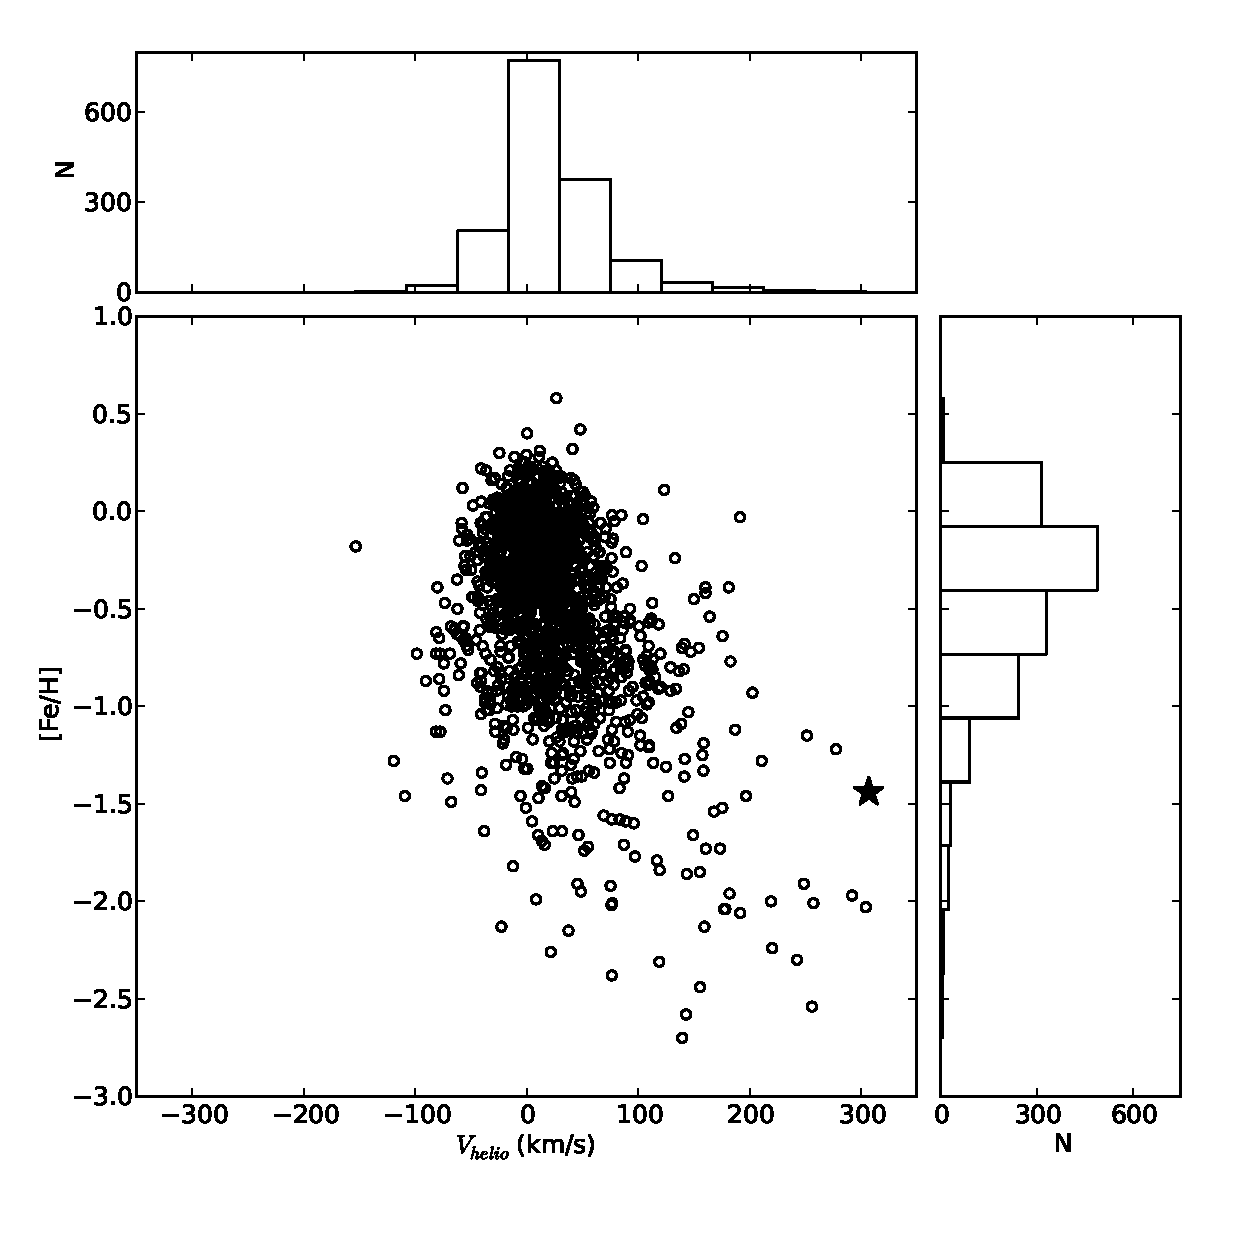
\includegraphics[width=\columnwidth]{besancon.eps}
  \caption{Kinematics and metallicities for representative halo stars from the Besan\c{c}on model \citep{Robin2003}. The star analysed here, Segue1-11, is marked as a filled star.}
  \label{fig:besancon}
\end{figure*}



\begin{figure*}
 \begin{center}
  \includegraphics{light_el.ps}
  \caption{Abundance ratios for light elements in Segue1-11 (filled star symbol), as measured from our high-resolution spectrum. For comparison, red and cyan points show thin and thick disk stars respectively, blue points show halo stars, and the crosses show stars in the classical dwarf galaxies Draco, Sextans, Ursa Minor, Carina, Fornax, Sculptor and Leo I. A typical error bar for our measurements is shown in the lower-left panel; also see Table~\ref{tab:seg11_sigma}. }
  \label{fig:light_el}
 \end{center}
\end{figure*} 


\begin{figure*}
 \begin{center}
  \includegraphics{nc_el.ps}
  \caption{Abundance ratios for the neutron-capture elements Sr, Ba, La and Eu in Segue1-11. Symbols as in Fig.~\ref{fig:light_el}.}
  \label{fig:nc_el}
 \end{center}
\end{figure*} 


\subsection{Metallicity of Stream}
We determine a metallicity of [Fe/H] $= -1.44 \pm XX $ for Segue1-11 based on the high-resolution spectrum. This is consistent with what we estimate from fitting globular cluster sequences to the photometry, and generally in agreement with the prediction of [Fe/H] $= -1.3$ from \citet{Simon2011}. It adds support to the result that the stream stars have higher metallicity than Segue\,1 system, as noted in S11 based on Ca triplet equivalents widths. The AAOmega sample of N10 contains some metallicity estimates based on CaII K line strengths; in addition to Segue1-11, the spectrum of the stream star Segue1-101 (SDSSJ100659.01+154418.8) has enough counts to yield [Fe/H] $\simeq -1.7$. Beyond this, we do not have data to determine the metallicity spread of the stream. 


\subsection{Abundance Ratios}
\label{sec:ab_rat}
Figures~\ref{fig:light_el} and \ref{fig:nc_el} show the abundance patterns of Segue1-11, based on our high-resolution spectrum. The blue, cyan and red points show stars in the halo, thick disk and thin disk respectively, from the sample of \citet{Fulbright2000, Fulbright2002} (as classified by \citealt{Venn2004}). Since the Fulbright sample does not include Cr, Sr and La measurements, comparison points  (halo stars) for these elements are taken from \citet{Lai2007} and \citet{Barklem2005}. In addition, the crosses show abundance patterns of stars in the classical dwarf galaxies Draco, Sextans, Ursa Minor, Carina, Fornax, Sculptor and Leo I \citep{Shetrone2001, Shetrone2003, Geisler2005, Aoki2009, Cohen2009}.

The abundance ratios of Segue1-11 overlap well with the general halo population at that metallicity, though as noted in Section~\ref{sec:abund} the $\alpha$- and particularly Mg abundances are on the low end. (The Sr abundance also appears low, but as discussed in Section~\ref{sec:abund}, this is likely not significant due to the noisy spectrum in this region.) On the other hand, the general abundance pattern is still closer to a typical halo star than to a classical dwarf spheroidal galaxy star. 


We note that these abundance patterns are important for interpreting the nature of the stream and its potential progenitor. Judging from this one star, it may be that this is the first stream with halo-like abundances. This predicament illustrates that a careful mapping of the region around Segue\,1 and the 300~km~s$^{-1}$ stream is of great importance. Only then can the nature of the 300~km~s$^{-1}$ stars be determined in more detail, and especially whether there are two different poulations at this high velocity: the halo, and the stream. Initial work on SDSS data to address this question hints that this region is more complex than assumed thus far. An attempt to decompose the many populations in the Segue\,1 region will be presented in a forthcoming paper (A. Jayaraman et al., in preparation).



\subsection{Distance to stream}

We use two different methods of estimating the distance to the stream. First, we interpolate the stellar parameters derived from the absorption lines onto the [Fe/H] $= -1.5$ isochrone shown in Fig.~\ref{fig:isochr}, extracting an inferred absolute magnitude $M_V \simeq +1.37$ for Segue1-11. Transforming from the Sloan photometry following \citet{Jordi2006}, and correcting for extinction according to \citet{Schlegel1998}, we find Segue1-11 has $V = 17.60$. This yields a distance modulus of $16.23$, resulting in a best distance estimate of $\simeq 18$ kpc. Given their uncertainty, however, a distance within $\pm 7$ kpc of this estimate would still be consistent with the stellar parameters derived from spectroscopy. Furthermore, our distance estimate of 18 kpc is in good agreement with \citet{Simon2011} who find a distance of 22 kpc to the stream.


A second distance estimate comes from using the photometric data and comparing the color-magnitude diagram to various globular cluster sequences from \citet{An2008}, shifted according to the distance moduli and reddenings compiled in \citet{Harris1996}. As seen in Fig.~\ref{fig:col_mag}, the M5 sequence is a good fit to the stream data when shifted to a distance of 18 kpc. This is in good agreement with the estimate based on spectroscopically determined stellar parameters.

Both the isochrone fit based on the single spectroscopic measurement and the photometric data indicate that the stream stars are at a distance of $\simeq 18$ kpc, slightly closer than the assumed distance of $23 \pm 2$ kpc \citep{Belokurov2007} for Segue\,1 itself. However, the uncertainties on both values are substantial enough that we cannot rule out that they are at the same distance. We also caution that since the stream stars were picked out in color-magnitude filters targeting stars at the distance of Segue1, the stream stars in our sample by design cannot be at a very different distance. 

We note that with galactic coordinates $l, b \simeq 220^{\circ}, 50^{\circ}$ and a heliocentric distance of 18 kpc, the stream stars are located in the outer galaxy. A heliocentric radial velocity of 300~km~s$^{-1}$ translates to Galactic Standard of Rest velocity of about 230~km~s$^{-1}$ in this direction, so the stream stars appear to be on a low angular momentum orbit that would eventually bring them far into the inner Galaxy.



\subsection{Origin of Stream}
We discuss here some possible scenarios regarding the origin of the stream.

\begin{itemize}
\item Since these high-velocity stars were discovered in a survey targeting Segue 1 members, a natural question to ask is whether the stream is related to the Segue\,1 dwarf galaxy. We find this an unlikely scenario for several reasons. First, the study of S11 finds no evidence that the Segue\,1 system is being tidally disrupted. Our distance estimate, based both on the high-resolution spectroscopy data and the photometry indicate that the stream stars are at a slightly closer distance than Segue\,1, though the data are not good enough to rule out that they are at the same distance. In addition, the color-magnitude diagrams suggest that the stream members are in general at a higher metallicity than Segue\,1, which our high-resolution measurement of one stream star also confirms. 

\item Another possibility, suggested by \citet{Geha2009}, is that these stars could be associated with the Sagittarius stream. Indeed at least two wraps of Sagittarius overlap with Segue 1 in this direction, and \citet{Niederste-Ostholt2009} argues that Segue 1 itself is a star cluster from the Sagittarius galaxy. But as for the stream stars, our metallicity measurement indicates that the 300~km~s$^{-1}$ stream does not have metallicities representative of Sgr debris, \citep{Chou2007, Casey2012}, and no Sgr debris model that we are aware of predicts a wrap at this velocity. Moreover, the part of the Sagittarius stream proposed to be contaminating Segue 1 samples has $v_{GSR} \sim 130$~km~s$^{-1}$ \citep{Niederste-Ostholt2009}, while the stream stars have $v_{GSR} \sim 230$~km~s$^{-1}$. 

\item The Orphan Stream \citep{Belokurov2007b} crosses the Sagittarius stream on the sky near Segue1, and at a similar distance modulus . Again, however, the velocities do not agree -- the reported velocities of the Orphan Stream are around $v_{GSR} \sim 110$~km~s$^{-1}$ \citep{Newberg2010}. In addition, the Orphan stream is metal-poor, with a reported mean metallicity of BHB stars [Fe/H] $ = -2.1$. Although both the Orphan Stream and Sagittarius Stream overlap with the 300~km~s$^{-1}$ stars, then, the combined metallicity and velocity information suggest that they are unrelated.

\item We have assumed throughout this paper that the 300~km~s$^{-1}$ feature is a stellar stream, but as pointed out in S11, until we can determine the full spatial extent of these stars, we cannot rule out that the stars belong to a bound object. If so, given the 1$^{\circ}$ extent seen in N10, its physical diameter would be at least 300 ($d / 18$ kpc) pc. This highlights the need for follow-up observations to map out the full extent of the 300~km~s$^{-1}$ stars.


\end{itemize}




%%%%%%%%%%%%%%%%%%%%%%%%%%%%%%%%%%%%%%%%%%%%%%%%%%%%%%%%%%%%%%%%%%%%%%%%%%%%%%%%%%%%%%%%%%%%%%%%%%%%%%

\section{Conclusions}
\label{sec:conc}
We have presented a high-resolution spectrum and abundance analysis of Segue1-11, a bright star in the 300~km~s$^{-1}$ stream near the ultra-faint dwarf galaxy Segue1. We determine a metallicity [Fe/H] $= -1.44 \pm XX$ for this star, with abundance ratios similar to typical halo stars at this metallicity. Fitting the stellar parameter solution onto theoretical isochrones, we estimate a distance of $18 \pm 7$ kpc. Both the metallicity and distance are in good agreement with estimates obtained from comparing the SDSS photometry to globular cluster sequences.

The fact that this stream may be largely chemically indifferent from the halo is particularly interesting. This is relevant to chemical tagging \citep{Freeman;Bland-Hawthorn2003}, which infers that stars originating from a common origin can be unambiguously identified solely by their chemistry and without the need for kinematics. This stream is most noticable only with its kinematics, and not by any particular chemical signature identified in this work. Although the luminosity, number of abundances analysed or abundance uncertainties presented here do not match the strict requirements for the complete chemical tagging planned in future galactic archaeology surveys \citep{Ting2012}, we identify this 300 km s$^{-1}$ stream as a candidate for testing and validating the chemical tagging concept. It would be particularly interesting to determine whether chemical tagging alone could identify members belonging to this 300 km s$^{-1}$ stream without the need for kinematics, as the chemical elements analysed here are only marginally distinguishable from the halo.

Although the 300~km~s$^{-1}$ stars are found in a region of sky with many known structures, the combination of velocity, chemistry and distance information makes it unlikely that these stars are associated with any of the Sagittarius stream, the Orphan stream, or the Segue\,1 dwarf galaxy. We therefore conclude that these stars belong to a new structure in the crowded ``Field of Streams''. Its features include an extreme mean velocity of 300~km~s$^{-1}$, a resolved and high velocity dispersion of 10~km~s$^{-1}$, a broad spatial distribution, and halo-like chemical abundances. The abundance patterns in particular make this stream very interesting to study in the context of halo formation. 

 

\section{Acknowledgements}
A.F. acknowledges support of a Clay Fellowship administered by the Smithsonian Astrophysical Observatory. A.R.C. acknowledges the financial support through the Australian Research Council Laureate Fellowship 0992131, and from the Australian Prime Minister's Endeavour Award Research Fellowship, which has facilitated his research at MIT. J.E.N. acknowledges support from the Australian Research Council (grants DP0663562, and DP0984924) for studies of the Galaxy's most metal-poor stars and ultra-faint satellite systems. R.F.G.W. acknowledges support from NSF grant AST-0908326.



%\bibliography{/home/rlunnan/myReferences}
\begin{thebibliography}{40}
\expandafter\ifx\csname natexlab\endcsname\relax\def\natexlab#1{#1}\fi

\bibitem[{{Abazajian} {et~al.}(2009){Abazajian}, {Adelman-McCarthy},
  {Ag{\"u}eros}, {Allam}, {Allende Prieto}, {An}, {Anderson}, {Anderson},
  {Annis}, {Bahcall}, \& et~al.}]{Abazajian2009}
{Abazajian}, K.~N., {et~al.} 2009, \apjs, 182, 543

\bibitem[{{An} {et~al.}(2008){An}, {Johnson}, {Clem}, {Yanny}, {Rockosi},
  {Morrison}, {Harding}, {Gunn}, {Allende Prieto}, {Beers}, {Cudworth},
  {Ivans}, {Ivezi{\'c}}, {Lee}, {Lupton}, {Bizyaev}, {Brewington},
  {Malanushenko}, {Malanushenko}, {Oravetz}, {Pan}, {Simmons}, {Snedden},
  {Watters}, \& {York}}]{An2008}
{An}, D., {et~al.} 2008, \apjs, 179, 326

\bibitem[{{Aoki} {et~al.}(2007){Aoki}, {Honda}, {Beers}, {Takada-Hidai},
  {Iwamoto}, {Tominaga}, {Umeda}, {Nomoto}, {Norris}, \& {Ryan}}]{Aoki2007b}
{Aoki}, W., {et~al.} 2007, \apj, 660, 747

\bibitem[{{Aoki} {et~al.}(2009){Aoki}, {Arimoto}, {Sadakane}, {Tolstoy},
  {Battaglia}, {Jablonka}, {Shetrone}, {Letarte}, {Irwin}, {Hill}, {Francois},
  {Venn}, {Primas}, {Helmi}, {Kaufer}, {Tafelmeyer}, {Szeifert}, \&
  {Babusiaux}}]{Aoki2009}
---. 2009, \aap, 502, 569

\bibitem[{{Asplund} {et~al.}(2009){Asplund}, {Grevesse}, {Sauval}, \&
  {Scott}}]{Asplund2009}
{Asplund}, M., {Grevesse}, N., {Sauval}, A.~J., \& {Scott}, P. 2009, \araa, 47,
  481

\bibitem[{{Barklem} {et~al.}(2005){Barklem}, {Christlieb}, {Beers}, {Hill},
  {Bessell}, {Holmberg}, {Marsteller}, {Rossi}, {Zickgraf}, \&
  {Reimers}}]{Barklem2005}
{Barklem}, P.~S., {et~al.} 2005, \aap, 439, 129

\bibitem[{{Belokurov} {et~al.}(2006){Belokurov}, {Zucker}, {Evans}, {Gilmore},
  {Vidrih}, {Bramich}, {Newberg}, {Wyse}, {Irwin}, {Fellhauer}, {Hewett},
  {Walton}, {Wilkinson}, {Cole}, {Yanny}, {Rockosi}, {Beers}, {Bell},
  {Brinkmann}, {Ivezi{\'c}}, \& {Lupton}}]{Belokurov2006b}
{Belokurov}, V., {et~al.} 2006, \apjl, 642, L137

\bibitem[{{Belokurov} {et~al.}(2007{\natexlab{a}}){Belokurov}, {Evans},
  {Irwin}, {Lynden-Bell}, {Yanny}, {Vidrih}, {Gilmore}, {Seabroke}, {Zucker},
  {Wilkinson}, {Hewett}, {Bramich}, {Fellhauer}, {Newberg}, {Wyse}, {Beers},
  {Bell}, {Barentine}, {Brinkmann}, {Cole}, {Pan}, \& {York}}]{Belokurov2007b}
---. 2007{\natexlab{a}}, \apj, 658, 337

\bibitem[{{Belokurov} {et~al.}(2007{\natexlab{b}}){Belokurov}, {Zucker},
  {Evans}, {Kleyna}, {Koposov}, {Hodgkin}, {Irwin}, {Gilmore}, {Wilkinson},
  {Fellhauer}, {Bramich}, {Hewett}, {Vidrih}, {De Jong}, {Smith}, {Rix},
  {Bell}, {Wyse}, {Newberg}, {Mayeur}, {Yanny}, {Rockosi}, {Gnedin},
  {Schneider}, {Beers}, {Barentine}, {Brewington}, {Brinkmann}, {Harvanek},
  {Kleinman}, {Krzesinski}, {Long}, {Nitta}, \& {Snedden}}]{Belokurov2007}
---. 2007{\natexlab{b}}, \apj, 654, 897

\bibitem[{{Bernstein} {et~al.}(2003){Bernstein}, {Shectman}, {Gunnels},
  {Mochnacki}, \& {Athey}}]{mike}
{Bernstein}, R., {Shectman}, S.~A., {Gunnels}, S.~M., {Mochnacki}, S., \&
  {Athey}, A.~E. 2003, in Society of Photo-Optical Instrumentation Engineers
  (SPIE) Conference Series, Vol. 4841, Society of Photo-Optical Instrumentation
  Engineers (SPIE) Conference Series, ed. {M.~Iye \& A.~F.~M.~Moorwood}, 1694

\bibitem[{{Casey} {et~al.}(2012){Casey}, {Keller}, {Da Costa}}]{Casey2012}
{Casey}, A. R., {et~al.} 2012, \aj, 143, 88

\bibitem[{{Cayrel} {et~al.}(2004){Cayrel}, {Depagne}, {Spite}, {Hill}, {Spite},
  {Fran{\c c}ois}, {Plez}, {Beers}, {Primas}, {Andersen}, {Barbuy},
  {Bonifacio}, {Molaro}, \& {Nordstr{\"o}m}}]{Cayrel2004}
{Cayrel}, R., {et~al.} 2004, \aap, 416, 1117

\bibitem[{{Cenarro} {et~al.}(2007){Cenarro}, {Peletier},
  {S{\'a}nchez-Bl{\'a}zquez}, {Selam}, {Toloba}, {Cardiel},
  {Falc{\'o}n-Barroso}, {Gorgas}, {Jim{\'e}nez-Vicente}, \&
  {Vazdekis}}]{Cenarro2007}
{Cenarro}, A.~J., {et~al.} 2007, \mnras, 374, 664

\bibitem[{{Chou} {et~al.}(2007){Chou}, {Majewski}, {Cunha}, {Smith},
  {Patterson}, {Mart{\'{\i}}nez-Delgado}, {Law}, {Crane}, {Mu{\~n}oz}, {Garcia
  L{\'o}pez}, {Geisler}, \& {Skrutskie}}]{Chou2007}
{Chou}, M.-Y., {et~al.} 2007, \apj, 670, 346

\bibitem[{{Cohen} \& {Huang}(2009)}]{Cohen2009}
{Cohen}, J.~G., \& {Huang}, W. 2009, \apj, 701, 1053

\bibitem[{{Frebel} {et~al.}(2010){Frebel}, {Simon}, {Geha}, \&
  {Willman}}]{Frebel2010a}
{Frebel}, A., {Simon}, J.~D., {Geha}, M., \& {Willman}, B. 2010, ApJ, 708, 560

\bibitem[{{Fulbright}(2000)}]{Fulbright2000}
{Fulbright}, J.~P. 2000, \aj, 120, 1841

\bibitem[{{Fulbright}(2002)}]{Fulbright2002}
---. 2002, \aj, 123, 404

\bibitem[{{Geha} {et~al.}(2009){Geha}, {Willman}, {Simon}, {Strigari}, {Kirby},
  {Law}, \& {Strader}}]{Geha2009}
{Geha}, M., {Willman}, B., {Simon}, J.~D., {Strigari}, L.~E., {Kirby}, E.~N.,
  {Law}, D.~R., \& {Strader}, J. 2009, \apj, 692, 1464

\bibitem[{{Geisler} {et~al.}(2005){Geisler}, {Smith}, {Wallerstein},
  {Gonzalez}, \& {Charbonnel}}]{Geisler2005}
{Geisler}, D., {Smith}, V.~V., {Wallerstein}, G., {Gonzalez}, G., \&
  {Charbonnel}, C. 2005, \aj, 129, 1428

\bibitem[{{Harris}(1996)}]{Harris1996}
{Harris}, W.~E. 1996, \aj, 112, 1487

\bibitem[{{Ibata} {et~al.}(1994){Ibata}, {Gilmore}, \& {Irwin}}]{Ibata1994}
{Ibata}, R.~A., {Gilmore}, G., \& {Irwin}, M.~J. 1994, \nat, 370, 194

\bibitem[{{Jordi} {et~al.}(2006){Jordi}, {Grebel}, \& {Ammon}}]{Jordi2006}
{Jordi}, K., {Grebel}, E.~K., \& {Ammon}, K. 2006, \aap, 460, 339

\bibitem[{{Kim} {et~al.}(2002){Kim}, {Demarque}, {Yi}, \&
  {Alexander}}]{Kim2002}
{Kim}, Y.-C., {Demarque}, P., {Yi}, S.~K., \& {Alexander}, D.~R. 2002, \apjs,
  143, 499

\bibitem[{{Kurucz}(1993)}]{kurucz}
{Kurucz}, R.~L. 1993, {Kurucz CD-ROM 13, ATLAS9 Stellar Atmosphere Programs and
  2 km/s Grid}, Cambridge: SAO

\bibitem[{{Lai} {et~al.}(2007){Lai}, {Johnson}, {Bolte}, \&
  {Lucatello}}]{Lai2007}
{Lai}, D.~K., {Johnson}, J.~A., {Bolte}, M., \& {Lucatello}, S. 2007, \apj,
  667, 1185

\bibitem[{{Lynden-Bell} \& {Lynden-Bell}(1995)}]{Lynden-Bell1995}
{Lynden-Bell}, D., \& {Lynden-Bell}, R.~M. 1995, \mnras, 275, 429

\bibitem[{{Majewski} {et~al.}(2003){Majewski}, {Skrutskie}, {Weinberg}, \&
  {Ostheimer}}]{Majewski2003}
{Majewski}, S.~R., {Skrutskie}, M.~F., {Weinberg}, M.~D., \& {Ostheimer}, J.~C.
  2003, \apj, 599, 1082

\bibitem[{{Newberg} {et~al.}(2010){Newberg}, {Willett}, {Yanny}, \&
  {Xu}}]{Newberg2010}
{Newberg}, H.~J., {Willett}, B.~A., {Yanny}, B., \& {Xu}, Y. 2010, \apj, 711,
  32

\bibitem[{{Niederste-Ostholt} {et~al.}(2009){Niederste-Ostholt}, {Belokurov},
  {Evans}, {Gilmore}, {Wyse}, \& {Norris}}]{Niederste-Ostholt2009}
{Niederste-Ostholt}, M., {Belokurov}, V., {Evans}, N.~W., {Gilmore}, G.,
  {Wyse}, R.~F.~G., \& {Norris}, J.~E. 2009, \mnras, 398, 1771

\bibitem[{{Norris} {et~al.}(2010){Norris}, {Wyse}, {Gilmore}, {Yong}, {Frebel},
  {Wilkinson}, {Belokurov}, \& {Zucker}}]{Norris2010a}
{Norris}, J.~E., {Wyse}, R.~F.~G., {Gilmore}, G., {Yong}, D., {Frebel}, A.,
  {Wilkinson}, M.~I., {Belokurov}, V., \& {Zucker}, D.~B. 2010, \apj, 723, 1632

\bibitem[{{Peterson}(1981)}]{Peterson1981}
{Peterson}, R.~C. 1981, \apj, 244, 989

\bibitem[{Robin} {et~al.}(2003){Robin}, {Reyl{\'e}}, {Derri{\`e}re}, \& {Picaud}]{Robin2003}
{Robin}, A.~C., 2003, \aap, 409, 523

\bibitem[{{Roederer} {et~al.}(2010){Roederer}, {Sneden}, {Thompson}, {Preston},
  \& {Shectman}}]{Roederer2010}
{Roederer}, I.~U., {Sneden}, C., {Thompson}, I.~B., {Preston}, G.~W., \&
  {Shectman}, S.~A. 2010, \apj, 711, 573

\bibitem[{{Schlegel} {et~al.}(1998){Schlegel}, {Finkbeiner}, \&
  {Davis}}]{Schlegel1998}
{Schlegel}, D.~J., {Finkbeiner}, D.~P., \& {Davis}, M. 1998, \apj, 500, 525

\bibitem[{{Shetrone} {et~al.}(2003){Shetrone}, {Venn}, {Tolstoy}, {Primas},
  {Hill}, \& {Kaufer}}]{Shetrone2003}
{Shetrone}, M., {Venn}, K.~A., {Tolstoy}, E., {Primas}, F., {Hill}, V., \&
  {Kaufer}, A. 2003, \aj, 125, 684

\bibitem[{{Shetrone} {et~al.}(2001){Shetrone}, {C{\^o}t{\'e}}, \&
  {Sargent}}]{Shetrone2001}
{Shetrone}, M.~D., {C{\^o}t{\'e}}, P., \& {Sargent}, W.~L.~W. 2001, \apj, 548,
  592

\bibitem[{{Simon} {et~al.}(2011){Simon}, {Geha}, {Minor}, {Martinez}, {Kirby},
  {Bullock}, {Kaplinghat}, {Strigari}, {Willman}, {Choi}, {Tollerud}, \&
  {Wolf}}]{Simon2011}
{Simon}, J.~D., {et~al.} 2011, \apj, 733, 46

\bibitem[{{Sneden}(1973)}]{moog}
{Sneden}, C.~A. 1973, PhD thesis, The University of Texas at Austin

\bibitem[{{Soubiran} {et~al.}(2008){Soubiran}, {Bienaym{\'e}}, {Mishenina}, \&
  {Kovtyukh}}]{Soubiran2008}
{Soubiran}, C., {Bienaym{\'e}}, O., {Mishenina}, T.~V., \& {Kovtyukh}, V.~V.
  2008, \aap, 480, 91

\bibitem[{{Ting} {et~al.}(2012){Ting}, {Freeman}, {Kobayashi}, {de Silva}, \& {Bland-Hawthorn}}]{Ting2012}
{Ting}, Y.~S., {Freeman}, K.~C., {Kobayashi}, C., {de Silva}, G.~M., \& {Bland-Hawthorn}, J.
 2012, \mnras, 421, 1231

\bibitem[{{Tolstoy} {et~al.}(2009){Tolstoy}, {Hill}, \& {Tosi}}]{Tolstoy2009}
{Tolstoy}, E., {Hill}, V., \& {Tosi}, M. 2009, ARA\&A, 47, 371

\bibitem[{{Venn} {et~al.}(2004){Venn}, {Irwin}, {Shetrone}, {Tout}, {Hill}, \&
  {Tolstoy}}]{Venn2004}
{Venn}, K.~A., {Irwin}, M., {Shetrone}, M.~D., {Tout}, C.~A., {Hill}, V., \&
  {Tolstoy}, E. 2004, \aj, 128, 1177

\end{thebibliography}





\end{document}

